% ------------------------------------------------------------------------------
% TYPO3 Version 10 LTS - What's New (English Version)
%
% @author	Michael Schams <schams.net>
% @license	Creative Commons BY-NC-SA 3.0
% @link		https://typo3.org/help/documentation/whats-new/
% @language	English
% ------------------------------------------------------------------------------

\section{Gebruikersinterface backend}
\begin{frame}[fragile]
	\frametitle{Gebruikersinterface backend}

	\begin{center}\huge{\color{typo3darkgrey}\textbf{Gebruikersinterface backend}}\end{center}
	\begin{center}\large{\textit{De TYPO3 beheersinterface is nu beter dan ooit}}\end{center}

\end{frame}

% ------------------------------------------------------------------------------
% ...

\begin{frame}[fragile]
	\frametitle{Gebruikersinterface backend}
	\framesubtitle{Backend UI wijzigingen}

	Enigszins gewijzigde UI van de kolom met modules.

	\begin{figure}
		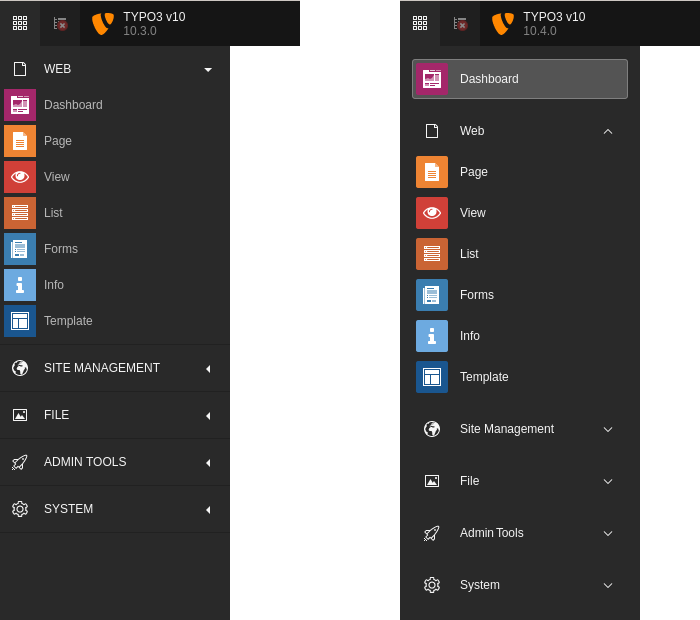
\includegraphics[width=0.5\linewidth]{BackendUserInterface/typo3-backend-ui.png}
	\end{figure}

\end{frame}

% ------------------------------------------------------------------------------
% Feature | 56213 | Allow sorting file list by file meta data title

\begin{frame}[fragile]
	\frametitle{Gebruikersinterface backend}
	\framesubtitle{Sortering bestandslijst}

	Bestanden kunnen gesorteerd wordt op de metadata-titel in het inhoudselement "Bestandskoppelingen".

	\begin{figure}
		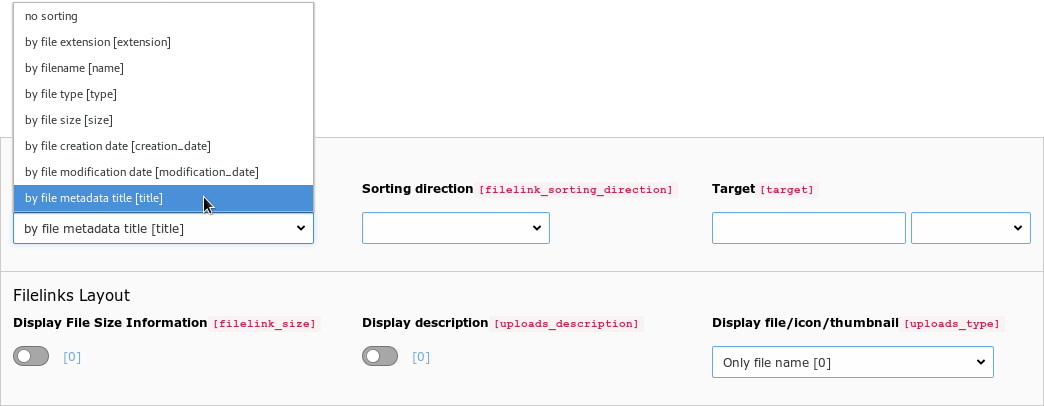
\includegraphics[width=0.90\linewidth]{BackendUserInterface/56213-FilelistSorting.png}
	\end{figure}

\end{frame}

% ------------------------------------------------------------------------------
% Feature | 85569 | Show scheduler information in the system information toolbar

\begin{frame}[fragile]
	\frametitle{Gebruikersinterface backend}
	\framesubtitle{Knoppenbalk systeeminformatie}

	De knoppenbalk systeeminformatie toont nu informatie over de TYPO3 taakplanner.

	\begin{figure}
		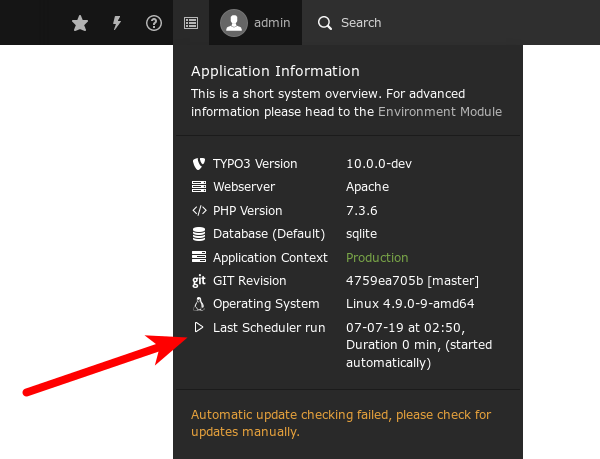
\includegraphics[width=0.50\linewidth]{BackendUserInterface/85569-SchedulerInfoInStatusBar.png}
	\end{figure}

\end{frame}

% ------------------------------------------------------------------------------
% Feature | 86629 | Implement LinkHandler for telephone numbers

\begin{frame}[fragile]
	\frametitle{Gebruikersinterface backend}
	\framesubtitle{Linkhandler}

	Een nieuwe linkhandler is toegevoegd waarmee redacteuren links kunnen maken naar
	telefoonnummers met het \texttt{tel:} protocol.

	\begin{figure}
		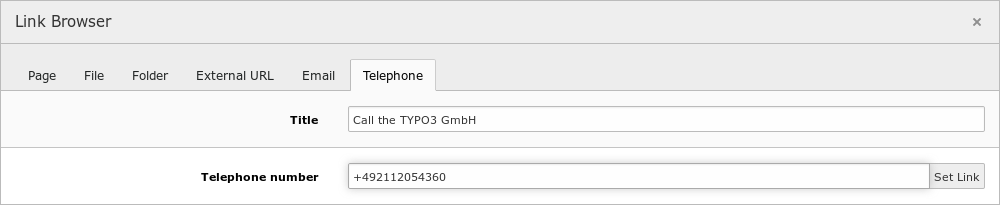
\includegraphics[width=0.90\linewidth]{BackendUserInterface/86629-TelephoneNumberLinkHandler.png}
	\end{figure}

	\begin{figure}
		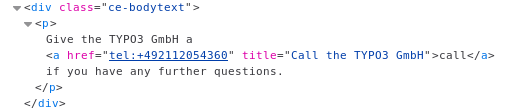
\includegraphics[width=0.60\linewidth]{BackendUserInterface/86629-TelephoneNumberLinkHandler2.png}
	\end{figure}

\end{frame}

% ------------------------------------------------------------------------------
% Feature | 87433 | Add changefreq and priority

\begin{frame}[fragile]
	\frametitle{Gebruikersinterface backend}
	\framesubtitle{\texttt{EXT:seo}: Backend Weergave}

	\texttt{EXT:seo} ondersteunt nu wijzigingsfrequentie en prioriteiten voor de sitemap.
	Pagina-eigenschappen (tab "SEO") bevat twee nieuwe velden.

	\begin{figure}
		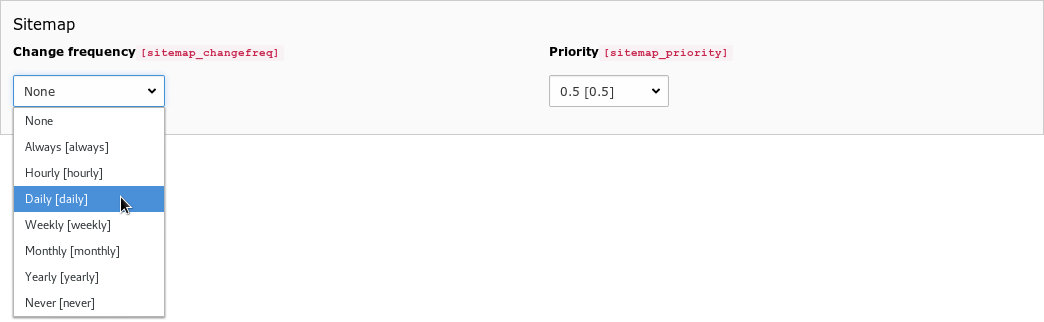
\includegraphics[width=0.90\linewidth]{BackendUserInterface/87433-SeoAddChangefreqAndPriority.png}
	\end{figure}

\end{frame}

% ------------------------------------------------------------------------------
% Feature | 87433 | Add changefreq and priority

\begin{frame}[fragile]
	\frametitle{Gebruikersinterface backend}
	\framesubtitle{\texttt{EXT:seo}: Configuratieopties voor Integrators}

	% decrease font size for code listing
	\lstset{basicstyle=\tiny\ttfamily}

	Deze instellingen kunnen ook in TypoScript gemaakt worden en worden overgezet naar velden
	in de database.

	\begin{lstlisting}
plugin.tx_seo {
  config {
    xmlSitemap {
      sitemaps {
        <unique key> {
          provider = TYPO3\CMS\Seo\XmlSitemap\RecordsXmlSitemapDataProvider
          config {
            ...
            changeFreqField = news_changefreq
            priorityField = news_priority
            ...
          }
        }
      }
    }
  }
}
	\end{lstlisting}

\end{frame}

% ------------------------------------------------------------------------------
% Feature | 83128 | Content Element Filter

\begin{frame}[fragile]
	\frametitle{Gebruikersinterface backend}
	\framesubtitle{Zoeken nieuw inhoudselement}

	Redacteuren kunnen zoeken naar inhoudselementen in de assistent "Nieuw inhoudselement":

	\begin{figure}
		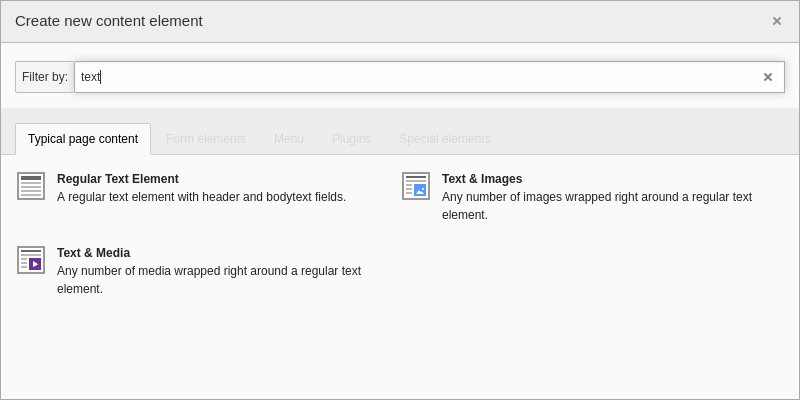
\includegraphics[width=0.6\linewidth]{BackendUserInterface/83128-ContentElementFilter.png}
	\end{figure}

\end{frame}

% ------------------------------------------------------------------------------
% Feature | 85918 | Hide in menu / Show in menu entry for pages in context menu

\begin{frame}[fragile]
	\frametitle{Gebruikersinterface backend}
	\framesubtitle{Tonen/verbergen in menu}

	In het contextmenu zit een nieuwe optie om pagina's te tonen/verbergen.

	\begin{figure}
		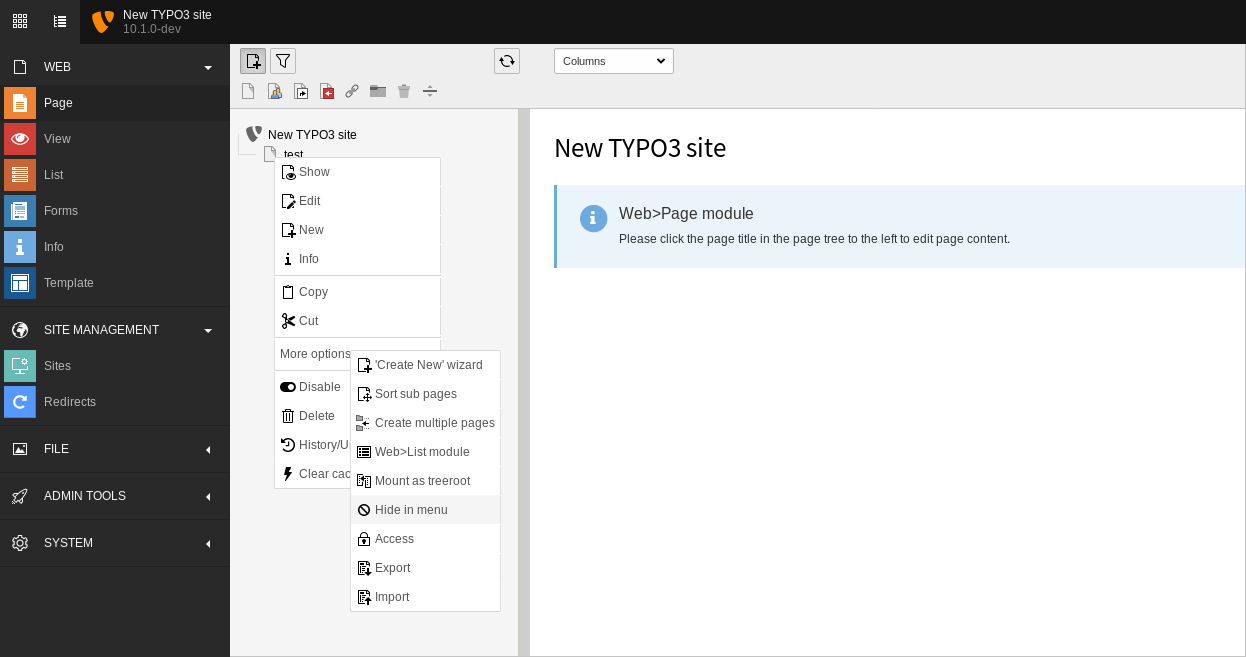
\includegraphics[width=0.80\linewidth]{BackendUserInterface/85918-HideShowInMenu-InContextMenu.png}
	\end{figure}

\end{frame}

% ------------------------------------------------------------------------------
% Feature | 89458 | Show link to online docs in extension manager

\begin{frame}[fragile]
	\frametitle{Gebruikersinterface backend}
	\framesubtitle{Extensie Manager}

	De module Extensies toont nu links naar de documentatie van de extensie.

	\begin{figure}
		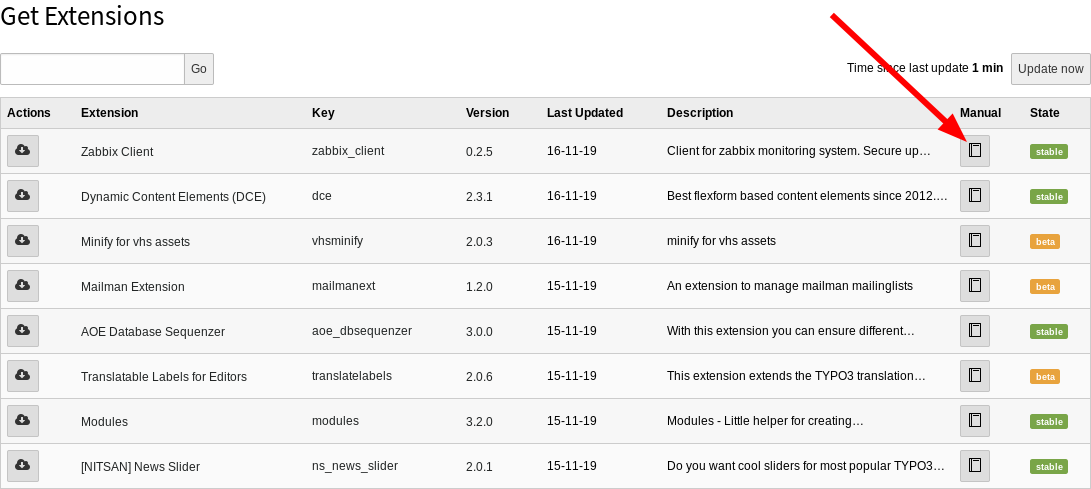
\includegraphics[width=0.90\linewidth]{BackendUserInterface/89458-ShowLinkToOnlineDocsInExtensionManager.png}
	\end{figure}

\end{frame}

% ------------------------------------------------------------------------------
% Feature | 89894 | Separate system extensions from 3rd-party extensions visually

\begin{frame}[fragile]
	\frametitle{Gebruikersinterface backend}
	\framesubtitle{Extensie Manager}

	Systeemextensies en extensies van derden kunnen nu apart getoond worden in de module Extensies.

	\begin{figure}
		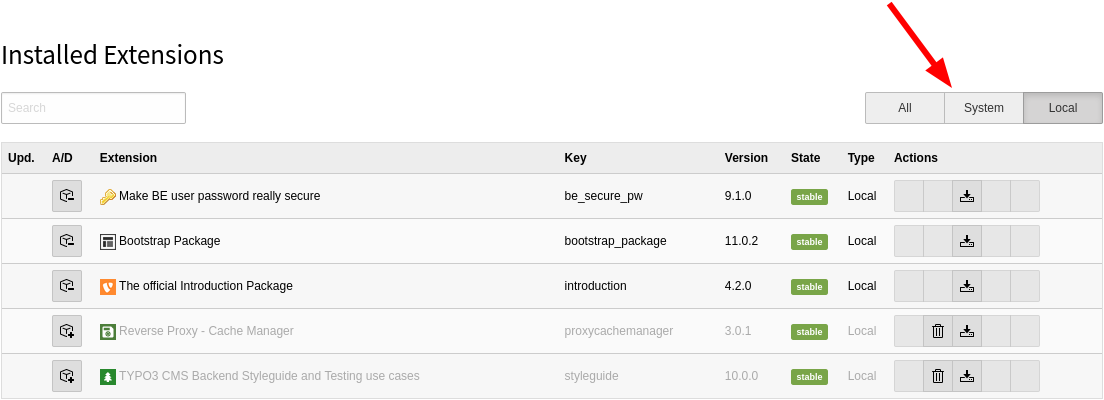
\includegraphics[width=0.9\linewidth]{BackendUserInterface/89894-SeparateSystemExtensionsFrom3rdPartyExtensionsVisually.png}
	\end{figure}

\end{frame}

% ------------------------------------------------------------------------------
% Feature | 86818 | Reintroduce keyboard accessible version of the pagetree

\begin{frame}[fragile]
	\frametitle{Gebruikersinterface backend}
	\framesubtitle{Toegankelijkheid paginaboom}

	Backend gebruikers kunnen nu hun toetsenbord gebruiken om te navigeren door de paginaboom.
	Toetsen die gebruikt kunnen worden zijn bijvoorbeeld de pijltjestoetsen, "home", "end", "enter", "space", etc.
	\newline
	Dit is gebaseerd op de adviezen die door de W3C zijn opgesteld in
	\href{https://www.w3.org/TR/wai-aria-practices-1.1/#keyboard-interaction-22}{WAI-ARIA Authoring Practices 1.1}.

	\begin{figure}
		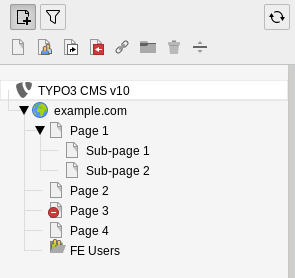
\includegraphics[width=0.30\linewidth]{BackendUserInterface/86818-PagetreeAccessibility.png}
	\end{figure}

\end{frame}

% ------------------------------------------------------------------------------
% Feature | 90298 | Improve user info in BE User module

\begin{frame}[fragile]
	\frametitle{Gebruikersinterface backend}
	\framesubtitle{Module backend-gebruikers}

	\begin{itemize}
		\item Een nieuwe detailweergave van backend-gebruikers toont alle relevante data.
		\item Extra velden zijn toegevoegd aan de functie voor het vergelijken van gebruikers.
		\item Deze functie kijkt nu ook naar subgroepen.
		\item Het uiterlijk van de module zal verder aangepast en geoptimaliseerd worden.
		\item Deze wijzigingen maken het makkelijker om gebruikers te controleren en te
		vergelijken zonder naar de gebruiker over te schakelen.
	\end{itemize}

\end{frame}

% ------------------------------------------------------------------------------
% Feature | 90826 | Compare backend usergroups

\begin{frame}[fragile]
	\frametitle{Gebruikersinterface backend}
	\framesubtitle{Module backendgebruikers}

	\begin{itemize}
		\item Integrators kunnen nu gebruikersgroepen vergelijken.
	\end{itemize}

	\begin{figure}
		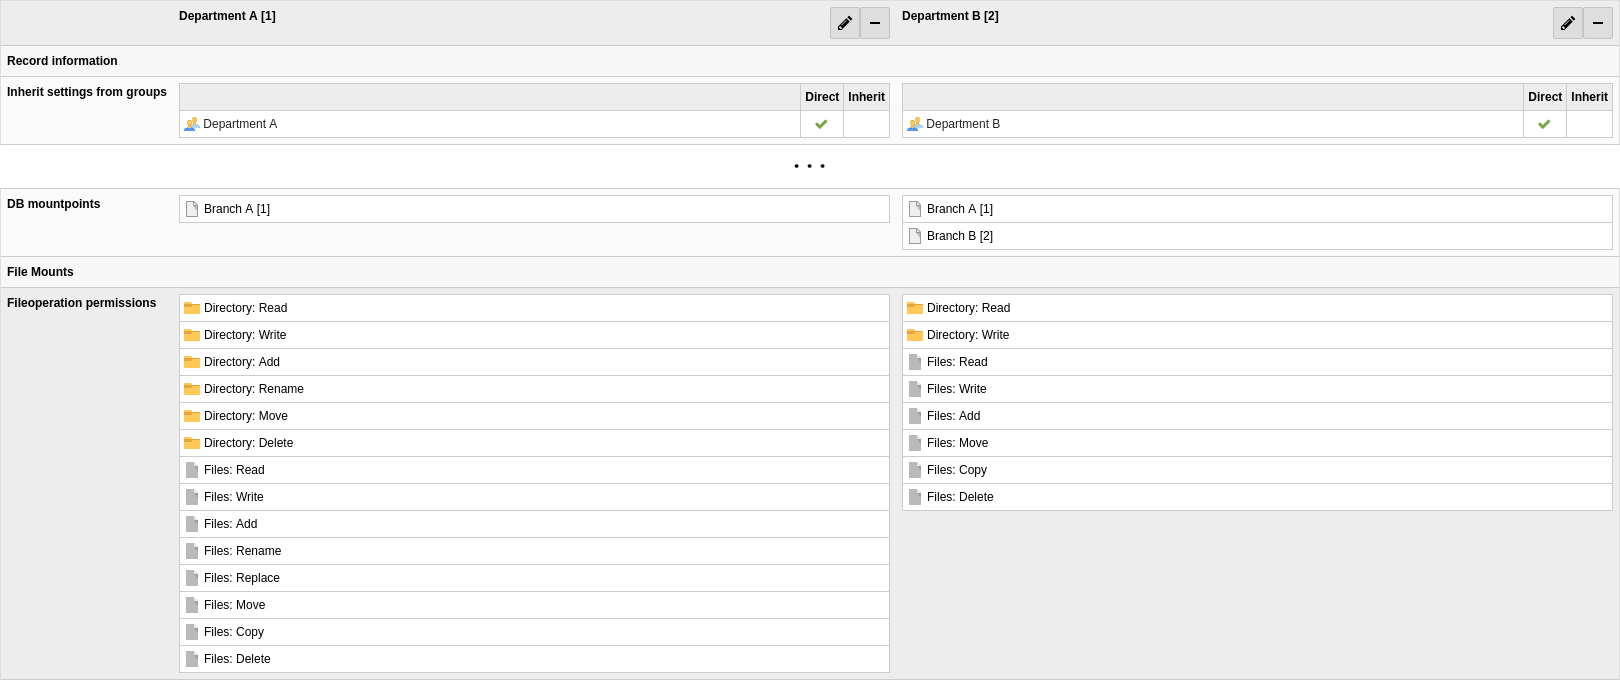
\includegraphics[width=0.9\linewidth]{BackendUserInterface/90826-CompareBackendUsergroups.png}
	\end{figure}

\end{frame}

% ------------------------------------------------------------------------------
% Feature | 90136 | Show application context in the Environment module

\begin{frame}[fragile]
	\frametitle{Gebruikersinterface backend}
	\framesubtitle{Overzicht omgeving}

	De huidige applicatiecontext wordt getoond in de module Omgeving:\newline
	\textbf{BEHEERWERKSET} $\rightarrow$ \textbf{Omgeving} $\rightarrow$ \textbf{Environment Overview}
% Environment Overview is part of the Install Tool and thus not translated

	\begin{figure}
		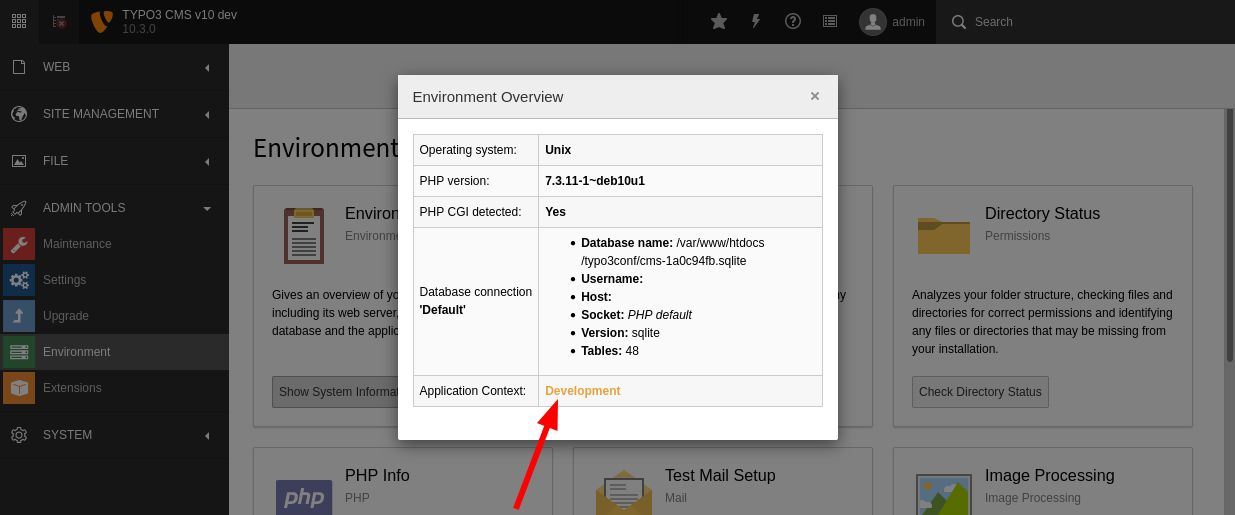
\includegraphics[width=0.9\linewidth]{BackendUserInterface/90136-ShowApplicationContextInTheEnvironmentModule.png}
	\end{figure}

\end{frame}

% ------------------------------------------------------------------------------
% Task | 89844 | Improve visual appearance of feature toggles

\begin{frame}[fragile]
	\frametitle{Gebruikersinterface backend}
	\framesubtitle{Optieschakelaars}

	De weergave van de optieschakelaars is verbeterd:
	\newline\newline
	\smaller\textbf{TYPO3 v9 LTS}\tabto{6cm}\textbf{TYPO3 v10 LTS}\normalsize

	\begin{figure}
		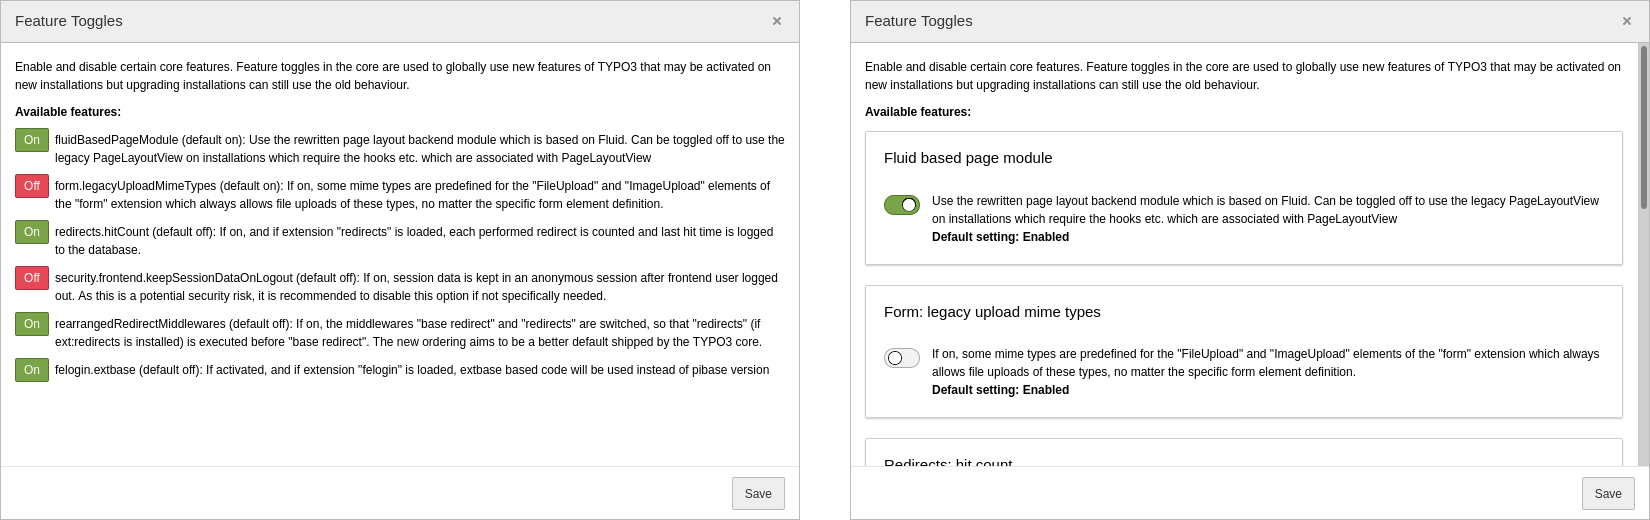
\includegraphics[width=1\linewidth]{InDepthChanges/89844-ImproveVisualAppearanceOfFeatureToggles.png}
	\end{figure}

\end{frame}

% ------------------------------------------------------------------------------
% Feature | 90425 | Add seo fields to info module

\begin{frame}[fragile]
	\frametitle{Gebruikersinterface backend}
	\framesubtitle{Infomodule}

	\begin{itemize}
		\item SEO en Sociale Media-details zijn toegevoegd aan de Infomodule:\newline
		\textbf{WEB} $\rightarrow$ \textbf{Info} $\rightarrow$ \textbf{Overzicht paginaboom}.
	\end{itemize}

	\begin{figure}
		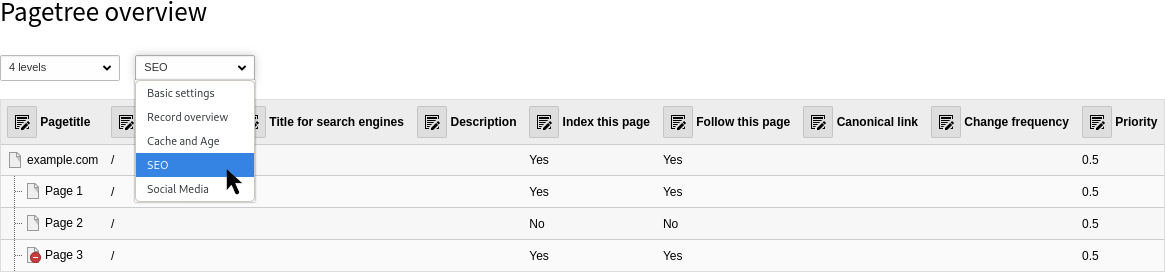
\includegraphics[width=0.85\linewidth]{BackendUserInterface/90425-AddSeoFieldsToInfoModule.png}
	\end{figure}

\end{frame}

% ------------------------------------------------------------------------------
% Feature | 89513 | Provide password recovery for backend users

\begin{frame}[fragile]
	\frametitle{Gebruikersinterface backend}
	\framesubtitle{Wachtwoord herstellen voor Backend-gebruikers}

	Backend-gebruikers kunnen nu een e-mail vragen voor het herstellen van hun wachtwoord.

	\begin{figure}
		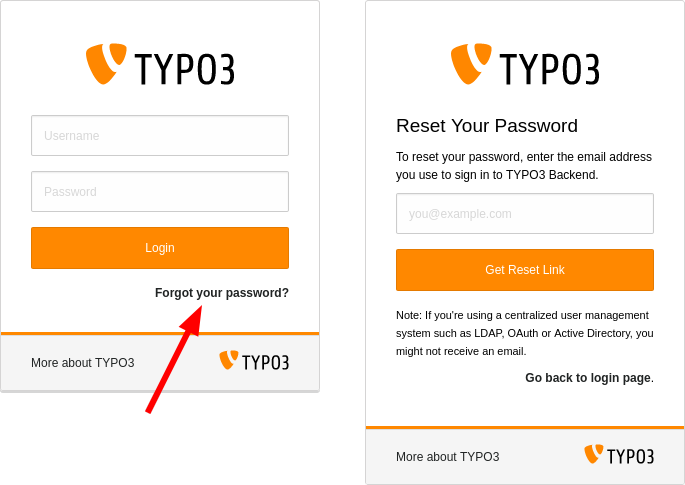
\includegraphics[width=0.55\linewidth]{BackendUserInterface/89513-ProvidePasswordRecoveryForBackendUsers.png}
	\end{figure}

\end{frame}

% ------------------------------------------------------------------------------
% Feature | 89513 | Provide password recovery for backend users

\begin{frame}[fragile]
	\frametitle{Gebruikersinterface backend}
	\framesubtitle{Wachtwoord herstellen voor Backend-gebruikers}

	\begin{itemize}

		\item E-mails voor het herstellen van wachtwoorden voor backend-gebruikers zijn maar 4 uur geldig.\newline
		Deze tijdslimiet is niet aanpasbaar.
		\item Voor betere beveiliging kan de functie uitgeschakeld worden voor admin-gebruikers of alle gebruikers.
		\item Als gebruikers hetzelfde e-mailadres hebben wordt een andere tekst gebruikt in de mail.
		\item TCA-veld \texttt{be\_users.email} mag niet ingesteld zijn op \texttt{eval=email}.

		\item De functie werkt alleen voor gebruikers, die:
			\begin{itemize}
				\item een e-mailadres ingesteld hebben,
				\item een wachtwoord ingesteld hebben en
				\item niet uitgeschakeld/verwijderd zijn.
			\end{itemize}

	\end{itemize}

\end{frame}

% ------------------------------------------------------------------------------
% Feature | 89513 | Provide password recovery for backend users

\begin{frame}[fragile]
	\frametitle{Gebruikersinterface backend}
	\framesubtitle{Wachtwoord herstellen voor Backend-gebruikers}

	\begin{itemize}
		\item E-mails voor herstellen van wachtwoorden kunnen ook via de commandoregel verstuurd worden.
	\end{itemize}

	\begin{figure}
		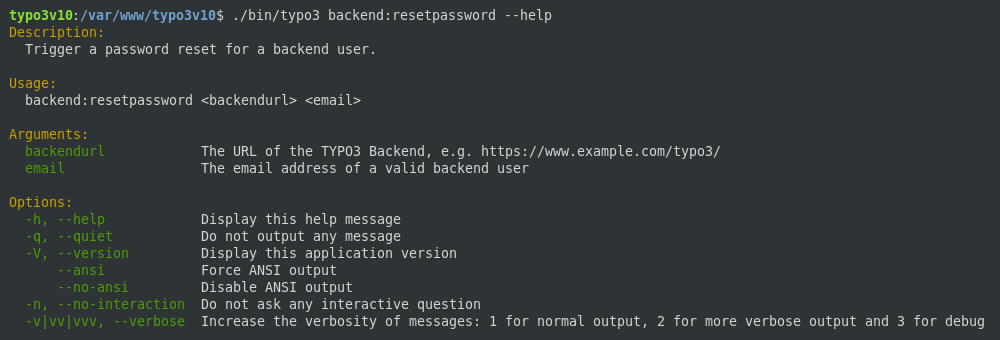
\includegraphics[width=0.9\linewidth]{BackendUserInterface/89513-BackendPasswordResetCommandLine.png}
	\end{figure}

\end{frame}

% ------------------------------------------------------------------------------
% Feature | 89115 | Auto slug update and redirect creation on slug change

\begin{frame}[fragile]
	\frametitle{Gebruikersinterface backend}
	\framesubtitle{Slug bijwerken en doorverwijzen}

	\begin{itemize}
		\item Als backendgebruikers het URL-pad van een pagina (zgn "slug") aanpassen
			is de oude URL niet meer beschikbaar.
		\item Dit resulteert mogelijk in een "pagina niet gevonden" melding voor deze
			pagina, inclusief de URL's van alle subpagina's.
	\end{itemize}

	\begin{figure}
		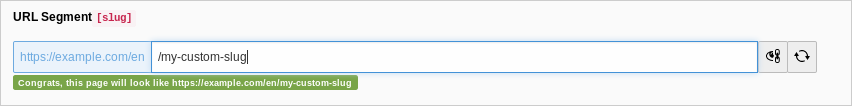
\includegraphics[width=0.80\linewidth]{BackendUserInterface/89115b-AutoSlugUpdateAndRedirectCreationOnSlugChange.png}
	\end{figure}

	\begin{itemize}
		\item Twee acties voorkomen dat dit gebeurt:

			\begin{itemize}
				\item slugs worden voor alle subpagina's automatisch bijgewerkt
				\item doorverwijzingen worden aangemaakt van de oude naar de nieuwe URL's
			\end{itemize}

	\end{itemize}

\end{frame}

% ------------------------------------------------------------------------------
% Feature | 89115 | Auto slug update and redirect creation on slug change

\begin{frame}[fragile]
	\frametitle{Gebruikersinterface backend}
	\framesubtitle{Slug bijwerken en doorverwijzen}

	\begin{itemize}
		\item Backendgebruikers krijgen een melding over deze acties en ze kunnen
			ze eenvoudig terugdraaien met een enkele klik:
	\end{itemize}

	\begin{figure}
		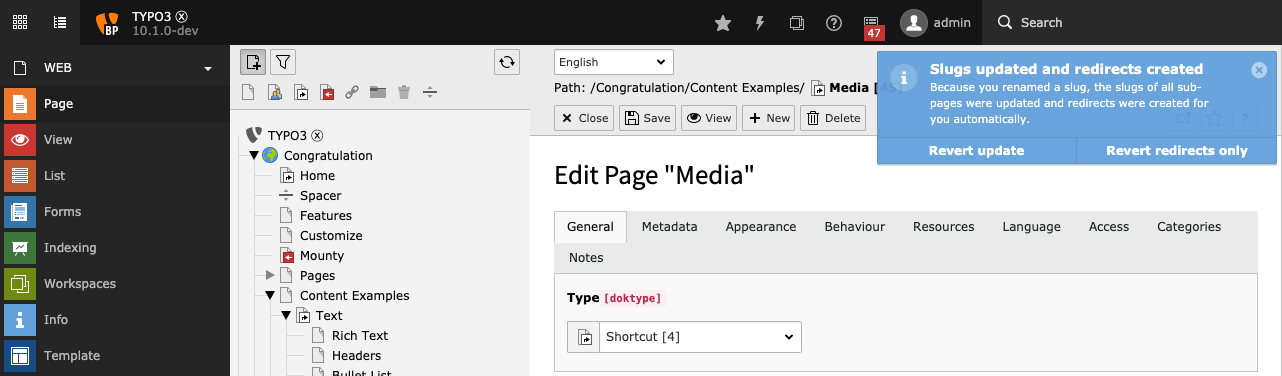
\includegraphics[width=0.80\linewidth]{BackendUserInterface/89115c-AutoSlugUpdateAndRedirectCreationOnSlugChange.png}
	\end{figure}

\end{frame}

% ------------------------------------------------------------------------------
